\documentclass[unicode,11pt,a4paper,oneside,numbers=endperiod,openany]{scrartcl}
\usepackage{amsmath}
\usepackage{listings}

\usepackage{ifthen}
\usepackage[utf8]{inputenc}
\usepackage{graphics}
\usepackage{graphicx}
\usepackage{hyperref}

\pagestyle{plain}
\voffset -5mm
\oddsidemargin  0mm
\evensidemargin -11mm
\marginparwidth 2cm
\marginparsep 0pt
\topmargin 0mm
\headheight 0pt
\headsep 0pt
\topskip 0pt        
\textheight 255mm
\textwidth 165mm

\newcommand{\duedate} {}
\newcommand{\setduedate}[1]{%
\renewcommand\duedate {\textbf{Due date:}~ #1}}
\newcommand\isassignment {false}
\newcommand{\setassignment}{\renewcommand\isassignment {true}}
\newcommand{\ifassignment}[1]{\ifthenelse{\boolean{\isassignment}}{#1}{}}
\newcommand{\ifnotassignment}[1]{\ifthenelse{\boolean{\isassignment}}{}{#1}}

\newcommand{\assignmentpolicy}{
\begin{table}[h]
\begin{center}
\scalebox{0.8} {%
\begin{tabular}{|p{0.02cm}p{16cm}|}
\hline
&\\
\multicolumn{2}{|c|}{\Large\textbf{Numerical Computing 2023 ---  Submission Instructions}}\\
\multicolumn{2}{|c|}{\large\textbf{(Please, notice that following instructions are mandatory: }}\\
\multicolumn{2}{|c|}{\large\textbf{submissions that don't comply with, won't be considered)}}\\
&\\
\textbullet & Assignments must be submitted to \href{https://www.icorsi.ch/course/view.php?id=14666}{iCorsi} (i.e. in electronic format).\\
\textbullet & Provide both executable package and sources (e.g. C/C++ files, MATLAB). 
If you are using libraries, please add them in the file. Sources must be organized in directories called:\\
\multicolumn{2}{|c|}{\textit{Project\_number\_lastname\_firstname}}\\
& and  the  file must be called:\\
\multicolumn{2}{|c|}{\textit{project\_number\_lastname\_firstname.zip}}\\
\multicolumn{2}{|c|}{\textit{project\_number\_lastname\_firstname.pdf}}\\
\textbullet &  The TAs will grade your project by reviewing your project write-up, and looking at the implementation you attempted, and benchmarking your code's performance.\\

\textbullet & You are allowed to discuss all questions with anyone you like; however: (i) your submission must list anyone you discussed problems with and (ii) you must write up your submission independently.\\
\hline
\end{tabular}
}
\end{center}
\end{table}
}
\newcommand{\punkte}[1]{\hspace{1ex}\emph{\mdseries\hfill(#1~\ifcase#1{Points}\or{Points}\else{Points}\fi)}}


\newcommand\serieheader[6]{
\thispagestyle{empty}%
\begin{flushleft}

\includegraphics[width=0.45\textwidth]{CI_logo}
\end{flushleft}
  \noindent%
  {\large\ignorespaces{\textbf{#1}}\hspace{\fill}\ignorespaces{ \textbf{#2}}}\\ \\%
  {\large\ignorespaces #3 \hspace{\fill}\ignorespaces #4}\\
  \noindent%
  \bigskip
  \hrule\par\bigskip\noindent%
  \bigskip {\ignorespaces {\Large{\textbf{#5}}}
  \hspace{\fill}\ignorespaces \large \ifthenelse{\boolean{\isassignment}}{\duedate}{#6}}
  \hrule\par\bigskip\noindent%  \linebreak
 }

\makeatletter
\def\enumerateMod{\ifnum \@enumdepth >3 \@toodeep\else
      \advance\@enumdepth \@ne
      \edef\@enumctr{enum\romannumeral\the\@enumdepth}\list
      {\csname label\@enumctr\endcsname}{\usecounter
        {\@enumctr}%%%? the following differs from "enumerate"
	\topsep0pt%
	\partopsep0pt%
	\itemsep0pt%
	\def\makelabel##1{\hss\llap{##1}}}\fi}
\let\endenumerateMod =\endlist
\makeatother




\usepackage{textcomp}







\begin{document}


\setassignment
\setduedate{Wednesday, 25 October 2023, 11:59 PM}

\serieheader{Numerical Computing}{2023}{Student: Hun Rim}{Discussed with: Georgy Batyrev}{Solution for Project 2}{}
\newline

\assignmentpolicy

\newpage

%%%%%%%%%%%%%%%%%%%%%%%%%%%%%%%%%%%%%%%%%%%%%%%%%%
\section{The assignment}
%%%%%%%%%%%%%%%%%%%%%%%%%%%%%%%%%%%%%%%%%%%%%%%%%%

\subsection{Implement various graph partitioning algorithms [50 points]}
The table below is a record of edgecuts calculated during the graph partitioning of various mesh graphs using various partitioning algorithms. \ref{table:bisection}.


\begin{table}[h]
\caption{Bisection results}
\centering
\begin{tabular}{l|r|r|r|r} \hline\hline 
Mesh             &  Coordinate           & Metis 5.0.2  & Spectral & Inertial  \\ \hline
grid5rec(12,100)&   12                   &      12       &     12     &       12    \\             
grid5rec(100,12)&   12                   &       12      &     12     &       12    \\ 
grid5recRotate(100,12,-45)&        22      &      12       &    12      &      12     \\ 
gridt(50)        &            72            &      82       &     78     &     72      \\ 
grid9(40)        &              118          &      127       &      140    &  118         \\ 
Smallmesh            &             25           &      12       &      14    &     30      \\ 
Tapir            &                55        &    23         &    58      &     49      \\ 
Eppstein            &              42          &       41      &    47      &   45        \\  
\hline \hline
\end{tabular}
\label{table:bisection}
\end{table}

Out of those 4 algorithms, 2 (Coordinate and Metis) were given whereas Spectral and Inertial had to be implemented. The following are the key factors of implementation for Spectral bisection according to the given psedo-code in the pdf file:\\

\begin{lstlisting}[language=Matlab]
    % 1. Construct the Laplacian.
    G = graph(A,'omitselfloops');
    L = laplacian(G);
    % 2. the correspoding vector of second smallest eigen value
    [V, ~] = eigs(L, 2, 'SM'); 
    % 3. Label the vertices with the components of the Fiedler vector.
    w = V(:,2);
    % 4. Partition them around their median value, or 0.
    threshold = median(w);
    part1 = find(w < threshold);
    part2 = find(w >= threshold);
\end{lstlisting}
\vspace{20px}
The code snippet below shows the implementation of Inertial bisection: \\

\begin{lstlisting}[language=Matlab]
    % 1. Calculate the center of mass (lets call it 'com').
    com = mean(xy);
    % 2. Construct the matrix M.
    Mxx = 0, Myy = 0, Mxy = 0;
    for i = 1:length(xy)
        Mxy = Mxy + (xy(i,1)-com(1))*(xy(i,2)- com(2));
        Myy = Myy + (xy(i,2)-com(2))^2;
        Mxx = Mxx + (xy(i,1)-com(1))^2;
    end
    M = [Mxx, Mxy; Mxy, Myy];
    % 3. Calculate the smallest eigenvector associated with M.
    [Eigenvector, Eigenvalue] = eigs(M);
    [~, minIndex] = min(diag(Eigenvalue));
    smallest = Eigenvector(:, minIndex);
    % 4. Find the line L on which the center of mass lies.
    L = smallest(1) * (xy(:,2) - com(2)) - smallest(2) * (xy(:,1) - com(1));
    % 5. Partition the points around the line L.
    medianL = median(L);
    part1 = find(L < medianL);
    part2 = find(L >= medianL);
 \end{lstlisting}

%----

\subsection{Recursively bisecting meshes [20 points]}

Result of recursive bi-partitioning for ${p = 8, l = 3}$ can be seen in Table \ref{table:Rec_bisection8}, and result for ${p = 16, l = 4}$ can be seen in Table \ref{table:Rec_bisection16}.

\begin{table}[h]
\caption{Edge-cut results for recursive bi-partitioning. ${p = 8, l = 3}$}
\centering
\begin{tabular}{l|r|r|r|r} \hline\hline 
 Case            &  Spectral             &  Metis 5.1.0    & Coordinate & Inertial  \\ \hline
 mesh3e1         &          58             &         57        &     63       &     59      \\             
 bodyy4        &              1093         &           985      &     1065       &      1364     \\ 
 de-2010            &         742              &        491         &  929          &     1084      \\ 
 biplane-9          &         510              &      465           &   548         &       648    \\ 
 L-9           &         705              &      637           &       631     &       828    \\  \hline \hline
\end{tabular}
\label{table:Rec_bisection8}
\end{table}


\begin{table}[h]
\caption{Edge-cut results for recursive bi-partitioning. ${p = 16, l = 4}$}
\centering
\begin{tabular}{l|r|r|r|r} \hline\hline 
 Case            &  Spectral             &  Metis 5.1.0    & Coordinate & Inertial  \\ \hline
 mesh3e1         &       58                &        57         &     63       &     59      \\             
 bodyy4        &        1839               &        1591         &   1951         &      2214     \\ 
 de-2010            &         1340              &        897         &  1796          &     2002      \\ 
 biplane-9          &         899              &        845         &   974         &      1093     \\ 
 L-9           &           1122            &        1019         &    1028        &      1377     \\  \hline \hline
\end{tabular}
\label{table:Rec_bisection16}
\end{table}

The results above are generated using the Bench\_rec\_bisection.m script. The following are the key implementations in the script: \\

\begin{minipage}{0.8\linewidth}

 \begin{lstlisting}[language=Matlab]
    %  @bisection_function: A pointer to function which carries out the 
    bisection. i.e. bisection_inertial.
    %  W: Original Square Matrix
    %  Coord: Given coordinates of the vertices.
    
    % Returns the map after the recursive bisection.
    recursiveBisection = rec_bisection(@bisection_function, log2(p), W,...
    coords, 0);
    
    % Returns the cutsize of the bisection.
    bisectCutSize = cutsize(W, recursiveBisection);
    
    % Plots the resulting map of a bisection
    gplotmap(W, coords, recursiveBisection);
  
 \end{lstlisting}
 \vspace{30px}

 {As it can be seen in the key implementations, the result of case 'de-2010' is visualized in the next page. } \\
  
\end{minipage}
\newpage

 \begin{figure}[h!]
    \begin{minipage}[c]{0.46\linewidth}
        \centering
        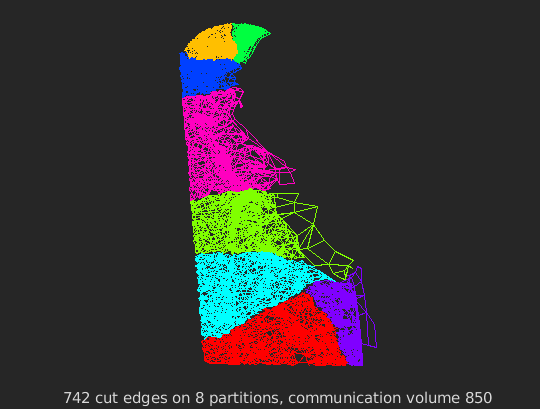
\includegraphics[width=0.8\linewidth]{./img/figure1.png}
    \end{minipage}
    \hfill%
    \begin{minipage}[c]{0.46\linewidth}
        \centering
        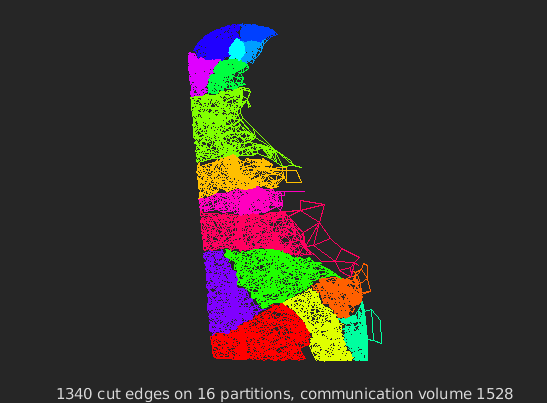
\includegraphics[width=0.8\linewidth]{./img/figure2.png}
    \end{minipage}
  \caption{Recursive Spectral Bisection ${p = 8, l = 3}$ left and ${ p = 16, l = 4}$ right}
  \label{fig:Another tiny Web}
\end{figure}

 \begin{figure}[h!]
  \begin{minipage}[c]{0.46\linewidth}
        \centering
        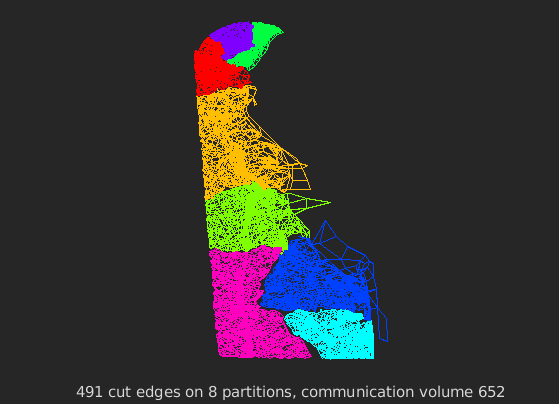
\includegraphics[width=0.8\linewidth]{./img/figure3.png}
    \end{minipage}
    \hfill%
    \begin{minipage}[c]{0.46\linewidth}
        \centering
        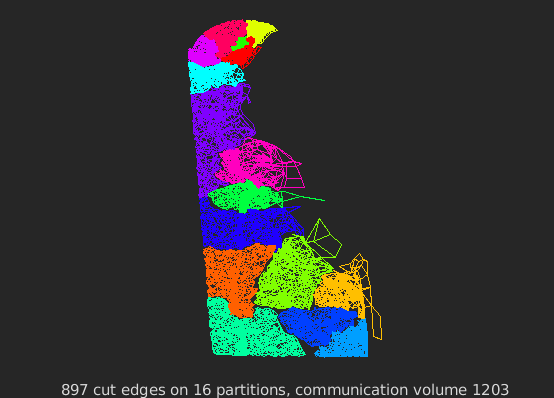
\includegraphics[width=0.8\linewidth]{./img/figure4.png}
    \end{minipage}
  \caption{Recursive Metis Bisection ${p = 8, l = 3}$ left and ${ p = 16, l = 4}$ right}
  \label{fig:Another tiny Web}
\end{figure}

 \begin{figure}[h!]
  \begin{minipage}[c]{0.46\linewidth}
        \centering
        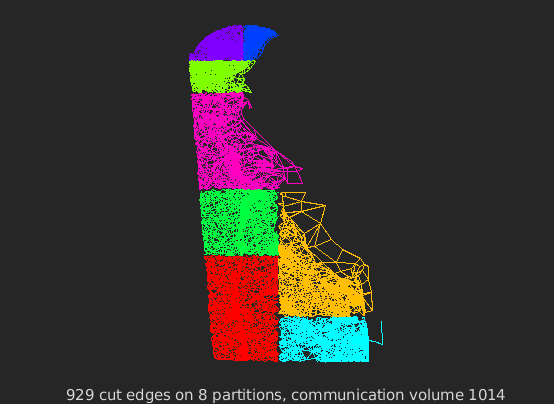
\includegraphics[width=0.8\linewidth]{./img/figure5.png}
    \end{minipage}
    \hfill%
    \begin{minipage}[c]{0.46\linewidth}
        \centering
        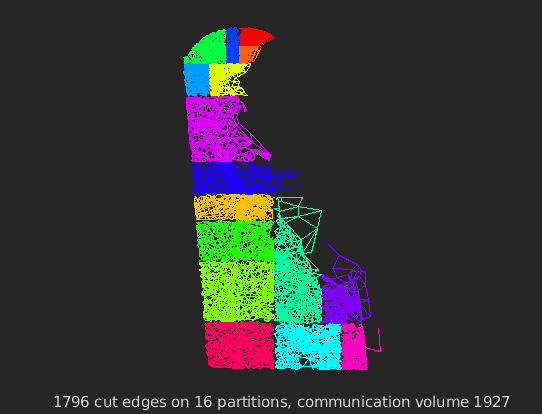
\includegraphics[width=0.8\linewidth]{./img/figure6.png}
    \end{minipage}
  \caption{Recursive Coordinate Bisection ${p = 8, l = 3}$ left and ${ p = 16, l = 4}$ right}
  \label{fig:Another tiny Web}
\end{figure}

 \begin{figure}[h!]
  \begin{minipage}[c]{0.46\linewidth}
        \centering
        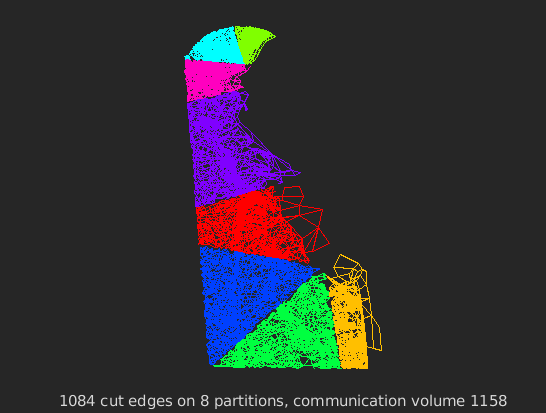
\includegraphics[width=0.8\linewidth]{./img/figure7.png}
    \end{minipage}
    \hfill%
    \begin{minipage}[c]{0.46\linewidth}
        \centering
        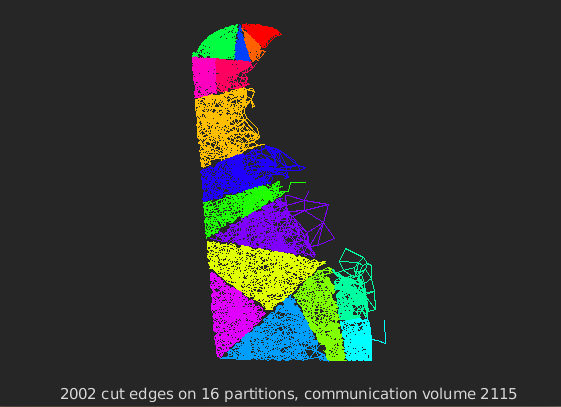
\includegraphics[width=0.8\linewidth]{./img/figure8.png}
    \end{minipage}
  \caption{Recursive Inertial Bisection ${p = 8, l = 3}$ left and ${ p = 16, l = 4}$ right}
  \label{fig:Another tiny Web}
\end{figure}

%----

\newpage

\subsection{Comparing recursive bisection to direct $k$-way partitioning [15 points]}

Results on table \ref{table:Compare_Metis} shows a similar performance as the number of edgecuts are very close to each other in all cases and the number of edge cuts almost doubled in all of the examples when the $k$ increased from 16 to 32. There might be some execution(calculation) time difference but number of edgecuts showed a very similar and predictable performance as suspected.

\begin{table}[h]
\caption{Comparing the number of cut edges for recursive bisection and direct multiway partitioning in Metis 5.1.0.}
\centering
\begin{tabular}{l|r|r} \hline\hline 
Partitions       &   Helicopter           & Skirt  \\ \hline
 16 - recursive bisection             &        343               &   3119  \\   
 16-way direct partition             &            324           &       3393      \\           
 32 - recursive bisection                &       537                &      6075       \\
 32-way direct partition              &            539           &       6051      \\  \hline \hline
\end{tabular}              
\label{table:Compare_Metis}
\end{table}
\vspace{20px}
The following are the visualization of ${helicopter}$ and ${skirt}$ models using different multiway partitioning methods given by the Metis 5.1.0. \\

 \begin{figure}[h!]
  \begin{minipage}[c]{0.46\linewidth}
        \centering
        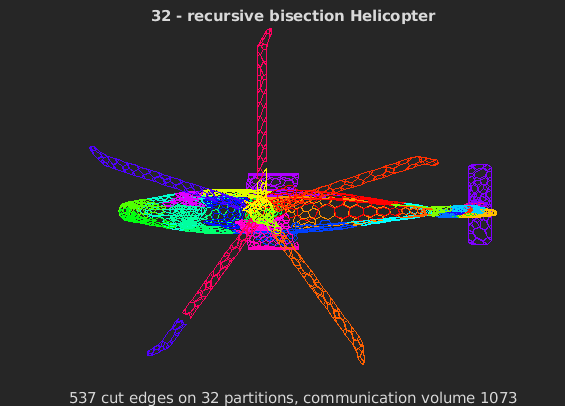
\includegraphics[width=0.8\linewidth]{./img/figure31.png}
    \end{minipage}
    \hfill%
    \begin{minipage}[c]{0.46\linewidth}
        \centering
        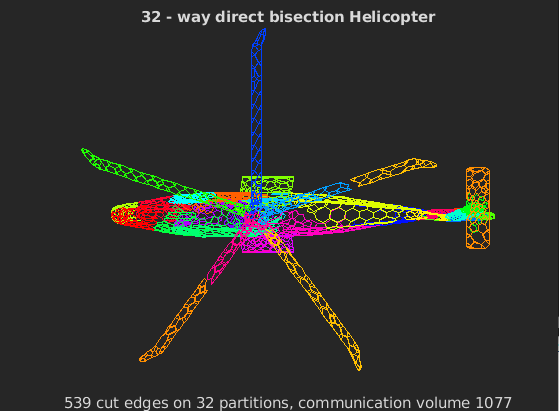
\includegraphics[width=0.8\linewidth]{./img/figure32.png}
    \end{minipage}
  \caption{Visualization of Helicopter using 32-recursive bisection (left) and 32-way direct bisection(right).}
  \label{fig:Another tiny Web}
\end{figure}

 \begin{figure}[h!]
  \begin{minipage}[c]{0.46\linewidth}
        \centering
        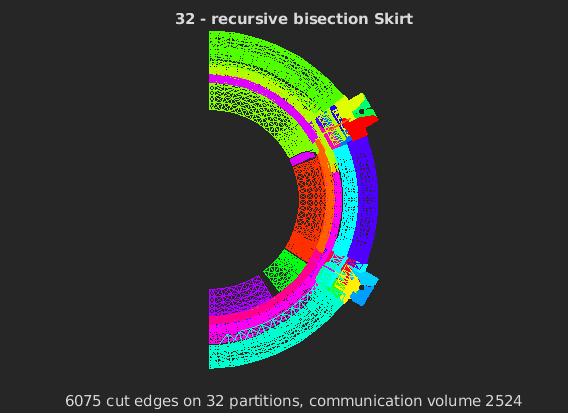
\includegraphics[width=0.8\linewidth]{./img/figure33.png}
    \end{minipage}
    \hfill%
    \begin{minipage}[c]{0.46\linewidth}
        \centering
        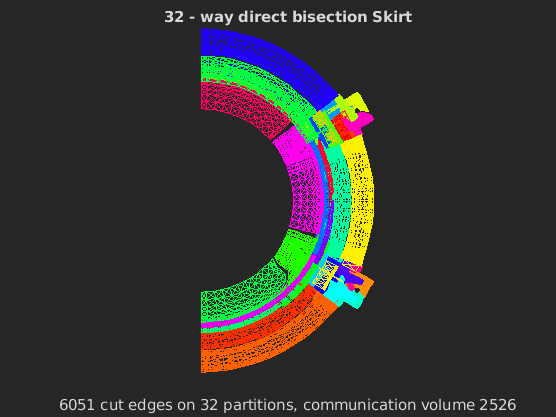
\includegraphics[width=0.8\linewidth]{./img/figure34.png}
    \end{minipage}
  \caption{Visualization of Skirt using 32-recursive bisection (left) and 32-way direct bisection(right).}
  \label{fig:Another tiny Web}
\end{figure}


The information on the table and visualization are obtained through running Bench\_metis.m script. In the next page are the key factors of implementation for the Bench\_metis.m script.

\newpage
 \begin{lstlisting}[language=Matlab]
    %To get a result of recursive bisection on MatrixA.
    [Map, edgeCutCount] = metismex('PartGraphRecursive', MatrixA, level);
    
    %To get a result of K-way bisection on MatrixA.
    [Map, edgeCutCount] = metismex('PartGraphKWay', MatrixA, level);
    
    %Resultant map of partition can be partitioned as the following
    gplotmap(MatrixA, CoordinatesA, Map);
    
    %To turn on the 3D view
    rotated3d on; % has to be called on a figure.
  
 \end{lstlisting}
{
 
 Please view the Bench\_metis.m script to see the full implementation of the task. The graphs generated from the script allows the viewer to rotate the graph around and view it in 3D perspective.
}
\end{document}
